\documentclass{beamer}

\usepackage[francais]{babel}
\usepackage[T1]{fontenc}
\usepackage[utf8]{inputenc}
\usepackage{enumerate}
\usepackage{listings}
\usepackage{xcolor}
\usepackage{graphicx}
\usepackage{geometry}
\usepackage{float}

\usetheme{Warsaw}

\title{Formats de Fichiers}
\author{Benjamin Vanthong}
\institute{Université de Strasbourg}


\lstdefinestyle{customjava}{
 belowcaptionskip=1\baselineskip,
 breaklines=true,
 %frame=single,
 %linewidth=7.5cm,
 %IMPORTANT marge
 framexleftmargin=0mm,
 %framexleftmargin=5mm,
 %frameround=tttt,
 %framexrightmargin=5mm,
 xleftmargin=\parindent,
 language=C++,
 showstringspaces=false,
 basicstyle=\footnotesize\ttfamily,
 keywordstyle=\color{green!40!black},
 ndkeywordstyle=\color{orange},
 commentstyle=\color{purple!40!black},
 identifierstyle=\color{blue},
 stringstyle=\color{red},
 %numbers=left,
 %numbersep=7pt,
}
\lstset{style=customjava, emph={int,double,void, Double}, emphstyle=\color{red}, emph={[2]wavJava, Spectrum}, emphstyle=[2]\color{orange}}

\begin{document}

\begin{frame}
\titlepage
\end{frame}

\section{Introduction}
\subsection {Objectifs du Stage}
\begin{frame}
\begin{itemize}
\item Implémenter un exportateur de solution aux formats HDF5 et XDMF pour la librairie \textbf{Feel++}
\item Implémenter une version permettant l'écriture parallèle dans ces formats
\end{itemize}
\end{frame}
\subsection{Description}
\begin{frame}
\begin{itemize}
\item Qu'est ce que Feel++ ?
\item Exportateurs existants :
\begin{itemize}
\item Format Gmsh (.msh)
\item Format EnSight Gold (.sos et .case)
\end{itemize}
\end{itemize}
\end{frame}

\begin{frame}
\tableofcontents[hideallsubsections]
\end{frame}
\section{HDF5}
\subsection{Description}
\begin{frame}
\frametitle {Description}
HDF5 (Hierarchical Data Format)
\begin{itemize}
\item Heavy Data
\item MPI (Message Passing Interface) intégré
\end{itemize}
Deux types d'objets :
\begin{enumerate}
\item ensemble de données appelés "dataset" : tableaux multidimmentionnels
\item "groups" : contiennent zéro ou plusieurs objets HDF5
\end{enumerate}
\end{frame}
\subsection{Fonctions}
\begin{frame}
\begin{itemize}
    \item Création d'un fichier : H5Fcreate
    \item Création d'un dataset : H5Dcreate
        \begin{itemize}
            \item datatype
            \item dataspace
        \end{itemize}
    \item Création d'un groupe  : H5Gcreate
        \begin{itemize}
            \item identfiant
            \item nom du groupe
        \end{itemize}
    \item Ecriture dans un dataset : H5Dwrite
\end{itemize}
Ne pas oublier de refermer les objets
\end{frame}
\subsection{La classe HDF5}
\begin{frame}[fragile]
\begin{itemize}
\item Simplification des entrées sorties
\item Implémentation des groupes
\begin{lstlisting}
void Feel::HDF5::createTable 
(const std::string& GroupName, 
const std::string& tableName, 
hsize_t tableDimensions[], 
const bool& existing)
\end{lstlisting}
\end{itemize}
\end{frame}
\subsection{Visualisation}
\begin{frame}
\begin{figure}
\begin{center}
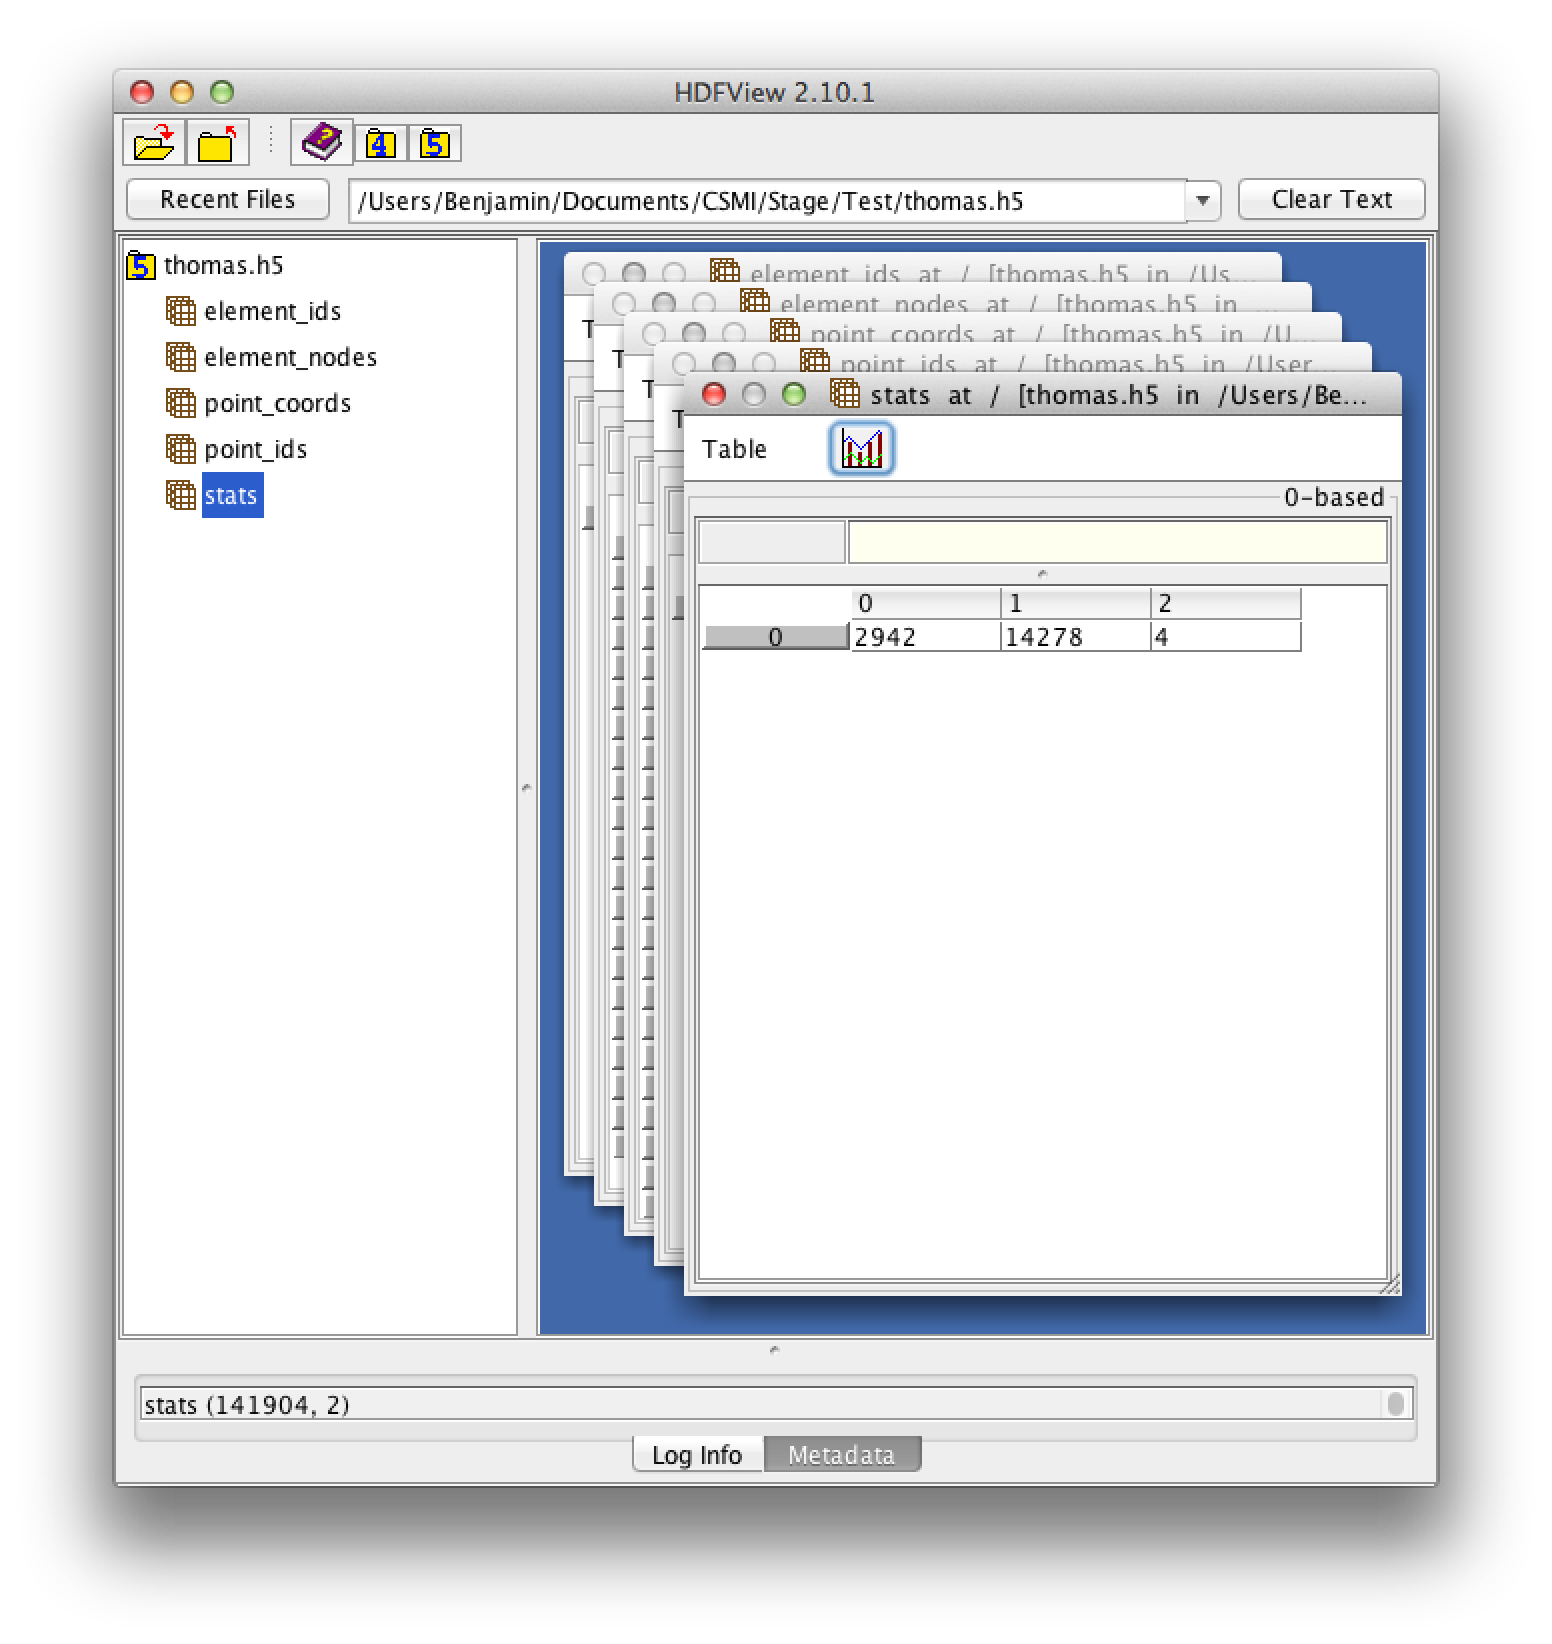
\includegraphics [width=\textwidth, height=\textheight] {HDFview.png}
\end{center}
\end{figure}
\end{frame}
\section{XDMF}
\subsection{Description}
\begin{frame}
\frametitle{Description}
XDMF (eXtensible Data Model and Format)
\begin{itemize}
\item accés aux données contenues dans un fichier HDF5
\item XML
\end{itemize}
\end{frame}
\subsection{Structure d'un fichier XDMF}
\begin{frame}[fragile]
Eléments :
\begin{verbatim}
<Nom element>
    Nom attribut = "Valeur"
    ...
</Nom element>
\end{verbatim}
\begin{itemize}
\item Domain
\item Grid
\item Topology
\item Geometry
\item Attribut
\item Time
\item DataItem
\end{itemize}
\end{frame}
\subsection{Exemple}
\begin{frame}[fragile, allowframebreaks]
\begin{lstlisting}[language=XML]
  <Domain>
    <Grid>
     <Geometry GeometryType="XYZ">
       <DataItem Dimension="50 3" NumberType="Float" Format="HDF" Precision="8">
         mylaplacian.h5:/points
       </DataItem>
     </Geometry>
     <Topology TopologyType="Triangle" NumberOfElements="102">
       <DataItem Dimension="102" NumberType="Int" Format="HDF" Precision="8">
         mylaplacian.h5:/nodes
       </DataItem>
     </Topology>
     <Attribute Name="temperature" AttributeType="Scalar" Center="Node">
        <DataItem Dimension="50 3" NumberType="Float" Format="HDF" Precision="8">
          mylaplacian.h5:/solutions
        </DataItem>
     </Attribute>
    </Grid>
  </Domain>
\end{lstlisting}
\end{frame}

\section{Exportateur}
\subsection{La classe Exporterhdf5}
\begin{frame}
\begin{itemize}
\item Classe Principale "Exporter"
\item --exporter.format=hdf5
\item Les Constructeurs
\end{itemize}
\end{frame}
\subsection{La méthode write}
\begin{frame}[fragile]
\frametitle{Algorithme de la méthode write}
\begin{verbatim} 
Ouverture du fichier XDMF
Parcours des pas de temps 
{
    Ouverture du fichier HDF5 pour un pas de temps donnee
    écriture des points
    écriture des éléments
    écriture des solutions
    Fermeture du fichier HDF5 pour ce pas de temps
}
Fermeture du fichier XDMF
\end{verbatim}
\end{frame}
\subsection{La méthode writePoint}
\begin{frame}[fragile]
\frametitle{Algorithme de la méthode writePoint}
\begin{enumerate} 
\item Création d'un dataset
\item Remplissage du buffer contenant les coordonnées des points 
\item Ecriture dans le dataset
\item Fermeture du dataset
\item Ecriture d'un bout de code XDMF associée à ce dataset
\end{enumerate}
\end{frame}
\subsection{La méthode writeElement}
\begin{frame}[fragile]
\frametitle{Algorithme de la méthode writeElement}
\begin{enumerate} 
\item Création d'un dataset
\item Remplissage du buffer d'éléments 
\item Ecriture dans le dataset
\item Fermeture du dataset
\item Ecriture d'un bout de code XDMF associée à ce dataset
\end{enumerate}
\end{frame}
\subsection{La méthode saveNodal}
\begin{frame}[fragile]
\frametitle{Algorithme de la méthode saveNodal}
\begin{verbatim} 
parcours de l'itérateur des solutions 
{
    Détermination du Type des solutions
    Création d'un dataset
    Remplissage du buffer 
    Ecriture dans le dataset
    Fermeture du dataset
    Ecriture d'un bout de code XDMF associée à ce dataset
}
\end{verbatim}
\end{frame}
\section{Parallélisation}
\begin{frame}
\begin{itemize}
\item Intérêt : Réduire les temps de calcul
\item Deux versions\newline
Utiliser l'option : --exporter.merge
\end{itemize}
\end{frame}
\subsection{Première version}
\begin{frame}
\begin{figure}
\begin{center}
%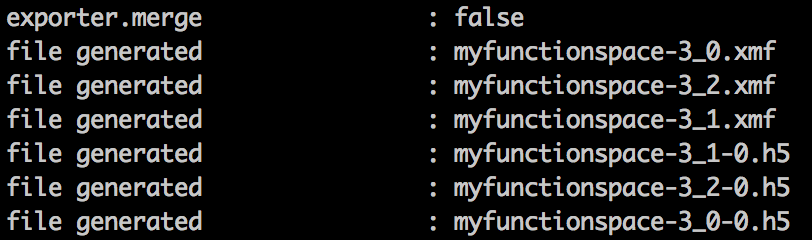
\includegraphics [width=\textwidth, height=\textheight-20] {Parallele1.png}
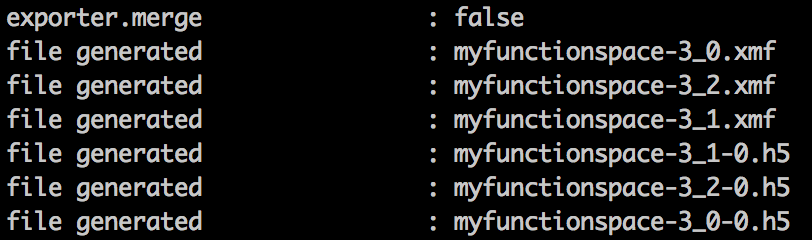
\includegraphics [width=\textwidth] {Parallele1.png}
\end{center}
\end{figure}
\end{frame}
\subsection{Deuxième version}
\begin{frame}
\frametitle{Fusion des fichiers}
Un seul fichier XDMF :\newline
\textcolor{blue}{
<Domain>\newline
    <Grid GridType="Collection" CollectionType="Spatial">\newline
    <Grid GridType="Uniform>\newline
    ...\newline
    </Grid>}\newline
\textcolor{red}{
    <Grid GridType="Uniform>\newline
    ...\newline
    </Grid>}\newline
\textcolor{green}{
    <Grid GridType="Uniform>\newline
    ...\newline
    </Grid>}\newline
\textcolor{blue}{
    </Grid>\newline
</Domain>}\newline
\end{frame}
\begin{frame}
\begin{figure}
%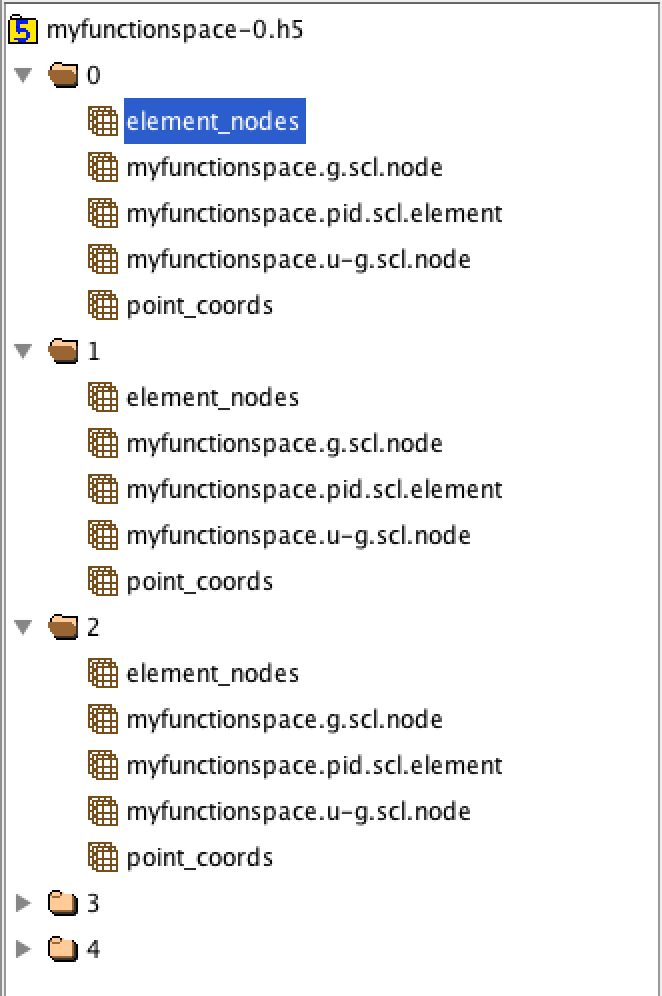
\includegraphics [width=\textwidth, height=\textheight] {HDFview5.png}
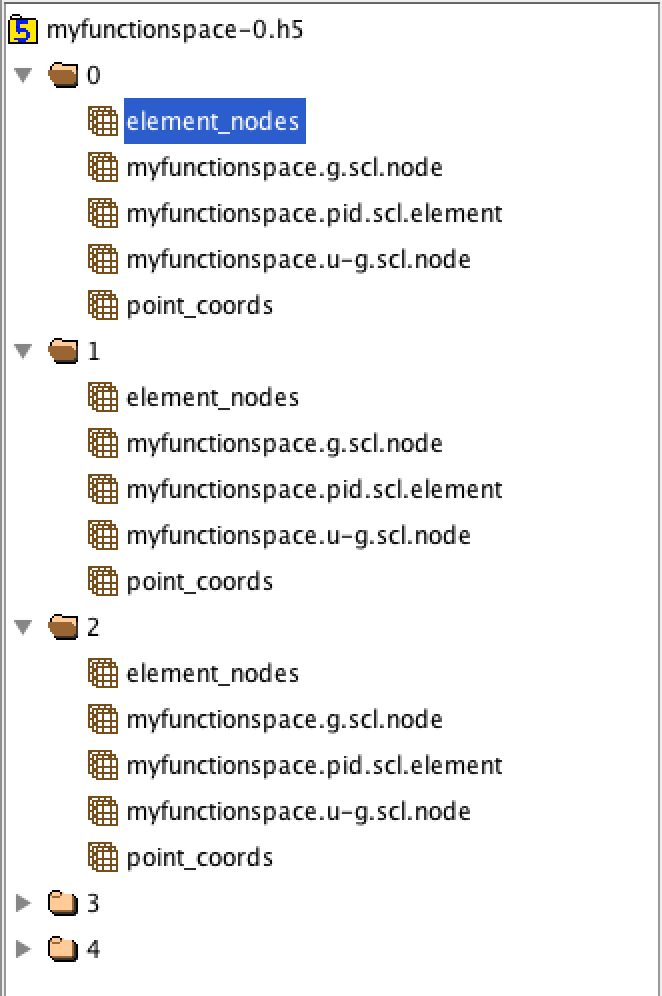
\includegraphics [scale=0.40] {HDFview5.png}
\end{figure}
\end{frame}
\subsection{Exemple}
\begin{frame}
\frametitle{maillage}
\begin{figure}
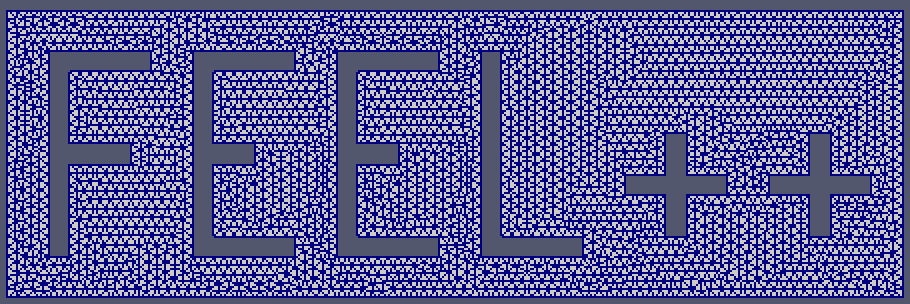
\includegraphics [width=\textwidth] {maillage.png}
\end{figure}
\end{frame}
\begin{frame}
\frametitle{Solution}
\begin{figure}

\includegraphics [width=\textwidth] {Feel1.png}
\end{figure}
\end{frame}
\begin{frame}
\frametitle{Partitionnement}
\begin{figure}

\includegraphics [width=\textwidth] {Feel3.png}
\end{figure}
\end{frame}
\section{Conclusion}
\begin{frame}
\begin{itemize}
\item Conclusions :
\begin{itemize}
\item Implémentation de l'export de solutions au format HDF5/XDMF
\item Parallélisation de l'exportateur
\end{itemize}
\item Perspectives :
\begin{itemize}
\item Faire des tests
\item Implémentation de l'importateur
\end{itemize}
\end{itemize}
\end{frame}

\end{document}

